% !TeX spellcheck = da_DK
\section{Systembeskrivelse}  

\subsection{Formål}
Systemet har til formål at gøre apopleksipatienter opmærksomme på, hvornår de mister balancen \fxnote{reference til problemafgrænsningen}. Systemet skal derfor kunne registrere, hvis patienten er i risiko for at falde og derved udsende et signal så patienterne har mulighed for at rette sig op igen. Selve systemet skal anvendes så patienterne er mere selvstændige i rehabiliteringsprocessen med henblik på at opnå en bedre balance. 

Det er på baggrund af afsnit.. valgt at hældningen på patienten skal opfanges via en sensor som er placeret på patienten. Systemet skal give visuelt feedback i form af to dioder, når patienten hælder til enten højre eller venstre. Når patienten hælder 5$^{\circ}$ til den ene side indikeres det af en gul diode, hvis patienten hælder yderligere, hvilket svarer til en hældning på 10$^{\circ}$ lyser en rød diode. Derudover anvendes sensorisk feedback via vibration som advarer patienten ved den gule diode og stiger i takt med at patienten hælder mere og mere.  

\subsection{Systemets bruger}
Systemet udvikles med henblik på selvtræning af balance i rehabiliteringsfasen. Derfor er systemets primære bruger patienten selv. Jævnfør afsnit (med apopleksipatienters alder) ses det at majoriteten af apopleksipatienter er over 65 år. Systemet skal være let anvendeligt så det kan anvendes af denne ældre demografi. Fagkyndigt personale, såsom fysioterapeuter og læger, skal kunne følge med i udviklingen som patienten gennemgår. Det skal derfor være muligt for disse også at benytte systemet. Dette gøres ved at systemet både har et analogt og digitalt output. Hvor det digitale henvender sig mere til et fagkyndigt personale.

\subsection{Anvendelse}
Systemet designes til at patienten under anvendelsen skal være stående på en tegnet linje med den ene fods tæer mod den anden fods hæl\fxnote{måske et billede vi tager som vil illustrere dette}. Denne position er valgt for at udfordre patientens balance ved at fordele kropsvægten anderledes ift. den normale kropsstilling omtalt på side \pageref{BalanceAfsnit}. Patienten påsætter selv systemet øverst på sternum og udfører herefter en kort prøvetest for at kende til de givne feedbackparametre. Under prøvetesten svajer patienten langsomt fra side til side. Hvis vedkommende hælder over 5$^{\circ}$, vil en gul diode lyse og vibrationen vil begynde. Hvis patienten svajer yderligere og hælder med over 10$^{\circ}$ vil en rød diode lyse. Vibrationen vil styrkes i takt med overgangen fra den gule til den røde diode. Efter testøvelsen udføres selve træningsøvelsen. Her indtages udgangspositionen på linjen og øjnene lukkes. Dette gøres for at udelukke den visuelle sans, hvilket gør det sværere for patienten at opretholde balancen. Patienten skal forsøge at holde balancen så længe som muligt uden at bevæge sig ud i risikozonerne, der vil blive markeret ved vibration. Træningsøvelsen gentages efter behov. \\
Ved at tage flere målinger igennem rehabiliteringsforløbet vil det forventes at der sker en fremgang ift. tiden hvori balancen kan opretholdes uden at patienten bevæger sig ud i risikozonerne. 

%\subsection{Accelerometer}
%I forsøget anvendes ADXL327 som er et tre-akset accelerometer ift. forsøget gives det elektriske signal ud fra X og Z-aksen. Produktet måler accelerationen med minimum fuldskala på \pm 2g. Sensitiviteten afhænger af forsyningsspændingen og ved 3V er sentivitivten 420mv/g. 

%Ledningerne snoes for at kontrollere samt mindske støjen. Derudover sættes ledninger fast med tape på patienten, så vidt det er muligt. For at undgå unødvendigt støj foretages forsøget væk fra andet elektronik.  %\ref{reference til støj afsnittet}

%\subsection{Analogt output}
%Det analoge output skal kunne henvende sig til patienten, dette sker ved lysdioder og vibration. Lysdioderne skal lyse gult ved 'usikkerhed' og slukke hvis patienten enten er rettet op igen eller bevæger sig ud i riskozonen, hvorefter en ny diode skal lyse rødt. Vibrationerne igangsættes ved 'usikkerhed' og skal stoppe hvis patienten retter sig op eller stige i styrke, hvis patienten kommer ud i risikozonen. 

%\subsection{Digitalt output}
%Det digitale skal kunne anvendes af sundhedspersonale til at vurdere om patienten gør fremskridt, dette indebærer at informationerne for patienten kan gemmes og sammenlignes på en computer. 


\subsection{Systemets opbygning}
Systemets opbygning fremgår af \figref{kravblok}.

\begin{figure}[H]
	\centering
	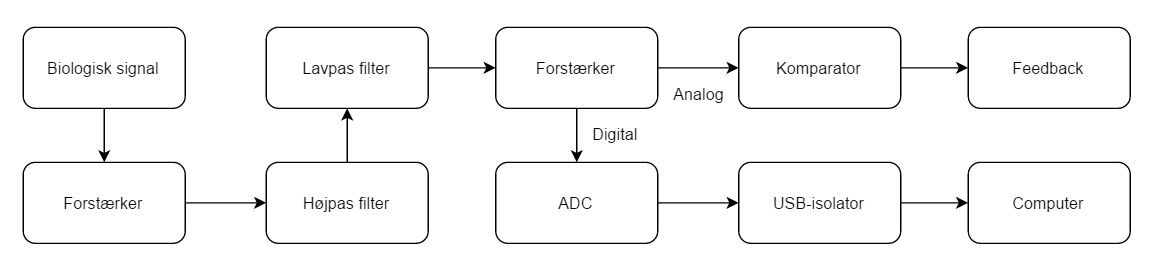
\includegraphics[scale=0.62]{figures/cProblemloesning/Systemopbygning.PNG}
	\caption{Figuren viser de blokke/elementer som systemet skal indeholde}
	\label{kravblok}
\end{figure}

Signalerne fra accelerometeret skal forstrækes, herefter støj skal filteres fra for at dæmpe uønskede frekvenser. Herefter forstærkes signalet med en variabel forstærkningen, da signalet kun er forstærket lidt. Signalet forstærkes til maksimalt 3V. Dette gøres ved en operationsforstærker \fxnote{inverteret eller ikke-inverteret} Det analoge signal ensrettet via. \fxnote{helbølgeensretter eller halvbølgeensretter}, hvor efter der benyttes en integrator til at lave en lineær linje. Ud fra denne linje gives en advarsel via feedback. Det digitale signal skal konverteres fra analogt til digitalt, hvilket gøres ved en ADC.  Herefter anvendes en USB-isolator for patientsikkerhed. Computeren skal fremvise en graf når NIDAQ er tilsluttet. 

\subsection{Kravspecifikationer}
Til vurdering af tolerance er der udført et pilotforsøg, dette er udført med henblik på at kunne beregne forstærkning, filtrering og integrering af signalet. 

\subsubsection{Det samlede system}
Det analoge output sammenligninger inputtet som kommer fra accelerometeret og outputtet i form af 2 dioder og stigning i vibration. Aktivering af bestemte dioder skal afspejle inputsignalet således at et lille input aktiverer en gul diode og vibration, mens et større input aktiverer en rød diode og stigningen i vibration. 

\textbf{Krav:}
\begin{itemize}
\item Den gule diode skal lyse når patienten har bevæget sig 5$^{\circ}$ og slukke hvis patienten retter sig op eller hælder yderligere.
\item Den røde diode skal lyse når patienten har bevæget sig 10$^{\circ}$ og slukke, hvis patienten retter sig op.
\item Vibration skal igangsættes når patienten har bevæget sig 5$^{\circ}$ og skal slukke, hvis patienten retter sig op eller stige, hvis patienten hælder yderligere.
\item Der skal være en sammenhæng mellem inputsignalets størrelse og antallet af dioder der lyser?
\item Signalet i systemet må ikke forstærkes til en værdi over 3V.
\end{itemize}

\subsection{Krav}
For at gøre anvendelse af samme system muligt til 4. Semester skal arbejdsområdet kunne benyttes sammen med et USB-baseret trådløst udviklingsværktøj eZ430-RF2500 fra Texas Instruments. Det er derfor nødvendigt, at designet stemmer overens med udviklingsværktøjet for at kunne sende og modtage data til og fra computeren. Udviklingsværktøjet indeholder hardware og software som evaluerer mikrokontrolleren MSP430F2274. For at hele vores system kan anvendes med udviklingsværktøjet, skal outputsignalet være 3V, eftersom mikrokontrolleren opererer med spændingsforsyning mellem 1,8V og 3,6V.

%\textbf{Tolerance:}
%\begin{itemize}
%\end{itemize}
%
%\subsubsection{Accelerometer}
%\textbf{Krav:}
%\begin{itemize}
%\end{itemize}
%
%\textbf{Tolerance:}
%\begin{itemize}
%end{itemize}
%
%\subsubsection{Instrumentering forstærker}
%\textbf{Krav:}
%\begin{itemize}
%\end{itemize}
%
%\textbf{Tolerance:}
%\begin{itemize}
%\end{itemize}
%
%\subsubsection{Filtre - opdeling i høj og lavpass?}
%\textbf{Krav:}
%\begin{itemize}
%\end{itemize}
%
%\textbf{Tolerance:}
%\begin{itemize}
%\end{itemize}

%\subsubsection{Forstærker med variabel forstærkning}

%\textbf{Krav:}
%\begin{itemize}
%\end{itemize}
%
%\textbf{Tolerance:}
%\begin{itemize}
%\end{itemize}
%
%\subsubsection{Ensretter}

%\textbf{Krav:}
%\begin{itemize}
%\end{itemize}
%
%\textbf{Tolerance:}
%begin{itemize}
%end{itemize}
%
%\subsubsection{Integrator}
%\textbf{Krav:}
%\begin{itemize}
%\end{itemize}
%
%\textbf{Tolerance:}
%\begin{itemize}
%\end{itemize}
%
%\subsubsection{Advarsel}
%\textbf{Krav:}
%\begin{itemize}
%\end{itemize}
%
%\textbf{Tolerance:}
%\begin{itemize}
%\end{itemize}
%
%\subsubsection{ADC}
%\textbf{Krav:}
%\begin{itemize}
%\end{itemize}
%
%\textbf{Tolerance:}
%\begin{itemize}
%\end{itemize}
%
%\subsubsection{USB-isolator}
%\textbf{Krav:}
%\begin{itemize}
%\end{itemize}
%
%\textbf{Tolerance:}
%\begin{itemize}
%\end{itemize}
%
%\subsubsection{Computer}
%\textbf{Krav:}
%\begin{itemize}
%\end{itemize}
%
%\textbf{Tolerance:}
%\begin{itemize}
%\end{itemize}
%\begin{itemize}
%\item Systemet skal ved fald få dioder til at lyse samt give feedback i form af stigende vibration. 
%\item Systemet skal være non-invasiv - dvs. systemet ikke må påføre patienten smerte eller varig skade
%\item Systemet skal være brugervenligt
%\item Systemet skal forsynes med spænding fra 9V batteri
%\end{itemize}

%\subsubsection{Accelerometer}
%Accelerometeret skal detektere patientens kropshældning.

%\subsubsection{Filter}
%Når der anvendes et filter, skal det dæmpe uønskede frekvenser. Dvs. frekvenser der lavere eller højere ift. det signal fra accelerometeret, som man vil analysere på. Der skal udføres et pilotforsøg for at finde frem til det korrekte filter og valg af knækfrekvens. 

%\subsubsection{Signalerende lys}
%Når patienten er ude af balance skal en rød diode lyse, som signalering ift. patientens hældning. Der skal vha. et pilotforsøg detekteres, hvornår dioden skal lyse. Skal der evt. være 2 dioder, hvor den ene er et "advarende" signal og nr. to er "fare". 

%\subsubsection{Alarm/vibrationen}
%Alarmen/vibrationen skal anvendes i perioden, hvor patienten er ude af balance og stoppe igen, når der igen er oprettet balance. 
%(eller fungere som en alarm til dioderne - så når en diode lyser, skal alarmen gå)

%\subsubsection{ADC}
%Der anvendes en ADC i systemet, for at konvertere det analoge signal til digitalt. Det næste skridt er konverteringen til PC og det er derfor essentielt at have en ADC, der konverterer analogt signal til binære tal, som digitale systemet anvender. 
%{Her skal vi have valgt en samplingsfrekvens)

%\subsubsection{USB-isolater}
%USB-isolatoren sikre patientens sikkerhed. Her skal input- og outputspænding være ens.  

%\subsubsection{Til PC}
%Fremvisning af graf, så patienten og plejepersonale kan følge %rehabiliteringens udvikling. 
